\documentclass[11pt,italian]{article}
\usepackage[T1]{fontenc}
\usepackage[utf8]{inputenc} %utf8 % lettere accentate da tastiera
\usepackage[italian]{babel} % lingua del documento
\usepackage{blindtext}
\usepackage{enumitem}
\usepackage{upquote}
\usepackage{float}
\usepackage{rotating}
\usepackage{xcolor}   % for \textcolor
\usepackage[font=small,labelfont=bf,skip=10pt]{caption}
\usepackage{subcaption}
\setlength{\belowcaptionskip}{5pt}
\usepackage{listings}
\lstset{
  basicstyle=\small\ttfamily,
  otherkeywords={self},             % Add keywords here
  basicstyle=\small\ttfamily,
  columns=fullflexible,
  frame=single,
  breaklines=true,
  postbreak=\mbox{\textcolor{red}{$\hookrightarrow$}\space},
  tabsize=4, % tab space width
  showstringspaces=false, % don't mark spaces in strings
  numbers=left, % display line numbers on the left
  commentstyle=\color[HTML]{a0a1a7}, % comment color
  keywordstyle=\color[HTML]{40a3f5}, % keyword color
  stringstyle=\color{red}, % string color,
  emphstyle={\color[HTML]{40a3f5}}
}
\usepackage{pythonhighlight}
\usepackage{hyperref}
\usepackage{cleveref}
\usepackage{graphicx}
\graphicspath{ {./images/} }

% Use lstinline as item in description
\makeatletter
\newcommand*{\lstitem}[1][]{%
  \setbox0\hbox\bgroup
    \patchcmd{\lst@InlineM}{\@empty}{\@empty\egroup\item[\usebox0]\leavevmode\ignorespaces}{}{}%
    \lstinline[#1]%
}
\makeatother

\title{Multiple Sequence Alignment (MSA) \\ di sequenze SARS-CoV-2}

\date{A.A.: 2019/2020}

\author{
    \textsc{Edoardo Silva} 816560 \\
    \textsc{Davide Marchetti} 815990
}

\begin{document}
\maketitle

\section{Abstract}
La seconda parte del progetto prevede di elaborare i file prodotti in precedenza ricavando informazioni relative alle alterazioni rilevate e producendo in output una tabella riassuntiva contenente:
\begin{itemize}
  \item il gene id del gene in cui cade la variazione con lo start e l'end della sua CDS rispetto alla reference
  \item il codone (o i codoni) alterato della reference, con posizione di inizio rispetto alla CDS, sequenza del codone e amminoacido codifcato
  \item il nuovo codone generato dalla variazione (o i nuovi codoni generati) specifcando la sequenza del codone e il nuovo amminoacido codifcato
\end{itemize}
Attraverso le informazioni raccolte in questa fase saremo in grado di identificare in quali geni si concentrano le variazioni rilevate, all'interno di essi, dove queste avvengono e come alterino i codoni causando la produzione di una proteina diversa.

\newpage
\section{Algoritmo}
L'algoritmo inizia caricando tutti i file necessari per l'elaborazione, in particolare quelli prodotti in output nella parte precedente del progetto:
\begin{enumerate}
  \item Caricamento della sequenza reference dal fasta corrispondente memorizzato in \lstinline{/project-1/input/reference.fasta}.
  \item Caricamento di uno dei file di output prodotti nella prima parte di progetto. Nel nostro caso è stato utilizzata l'analisi dell'allineamento di \lstinline{ClustalW}.
  \item Lettura del file \lstinline{Genes-CDS.xlsx} contenente le informazioni sui geni e le CDS della sequenza di reference. In particolare, una delle CDS analizzate derivava dall'unione (join) di due sequenze. In tal caso è possibile specificare il punto di unione della sequenza.
\end{enumerate}

\newpage
\section{Listati di codice}
\begin{lstlisting}[language=Python,caption=Tabella per la traduzione in amminoacidi,label=code:aminoacids_table]
aminoacids_lookup_table = {
  'F': ['TTT', 'TTC'],
  'L': ['TTA', 'TTG', 'CTT', 'CTA', 'CTC', 'CTG'],
  'I': ['ATT', 'ATC', 'ATA'],
  'M': ['ATG'],
  'V': ['GTT', 'GTA', 'GTC', 'GTG'],
  'S': ['TCT', 'TCA', 'TCC', 'TCG', 'AGT', 'AGC'],
  'P': ['CCT', 'CCA', 'CCC', 'CCG'],
  'T': ['ACT', 'ACA', 'ACC', 'ACG'],
  'A': ['GCT', 'GCA', 'GCC', 'GCG'],
  'Y': ['TAT', 'TAC'],
  'H': ['CAT', 'CAC'],
  'Q': ['CAA', 'CAG'],
  'N': ['AAT', 'AAC'],
  'K': ['AAA', 'AAG'],
  'D': ['GAT', 'GAC'],
  'E': ['GAA', 'GAG'],
  'C': ['TGT', 'TGC'],
  'W': ['TGG'],
  'R': ['CGT', 'CGA', 'CGC', 'CGG', 'AGA', 'AGG'],
  'G': ['GGT', 'GGA', 'GGC', 'GGG'],
  'START': ['ATG'],
  'STOP': ['TAA', 'TAG', 'TGA']
}
\end{lstlisting}

\newpage
\begin{lstlisting}[language=Python,caption=Memorizzazione dei risultati nella struttura dati a lista,label=code:variation_loop]
  for key, value in variations:
    for index, cds in affected_cdses.iterrows():
      ...
      variations_to_genes.append({
        'gene_id': gene_id,
        'gene_start': gene_start + 1, # 1-based position
        'gene_end': gene_end,
        'cds_start': cds_start + 1, # 1-based position
        'cds_end': cds_end,
        'original_codone': original_codone,
        'altered_codone': altered_codone,
        'relative_start': relative_start + 1, # 1-based position
        'relative_end': relative_end,
        'alteration': sequence,
        'original_aminoacid': original_aminoacid,
        'encoded_aminoacid': encoded_aminoacid
      })
\end{lstlisting}

\noindent
Dopo la lettura del materiale rilevante a questa fase di elaborazione, l'algoritmo itera le variazioni rilevate nell'allineamento e per ciascuna di esse esegue i seguenti step:
\begin{enumerate}
  \item Identifica le CDS nelle quali avviene l'alterazione rispetto alla reference.
  \item Recupera le informazioni del gene associato alle CDS rilevate calcolando le posizioni globali e relative alla CDS dell'alterazione.
  \item Identifica i codoni alterati e ne effettua la ritraduzione in amminoacidi grazie ad una look-up table (listato \ref{code:aminoacids_table}). Vengono ignorate le alterazioni che presentano sequenze di soli \lstinline{-}, derivate probabilmente da un sequenziamento errato o un'alterazione posta ai capi dell'allineamento.
  \item Memorizza tutte le informazioni ricavate in una struttura dati apposita tramite cui derivare la tabella per l'output finale associando i valori a chiavi prestabilite.
\end{enumerate}

\noindent
Al termine dell'elaborazione di tutte le alterazioni, viene costruito un oggetto di tipo \lstinline{DataFrame} fornito dalla libreria \lstinline{pandas}.

Le chiavi utilizzate nella costuzione della struttura dati a lista diventeranno le colonne del \lstinline{DataFrame}. Questo sarà esportato in CSV nella cartella \lstinline{/project-2/output/alteration-table.csv} per permettere una visualizzazione più semplice tramite programmi terzi (come riportato in \cref{fig:alteration_table})

\newpage
\section{Informazioni memorizzate}
Ad ogni variazione analizzata corrisponde un entrata nella struttura dati a lista contenente le seguenti informazioni:
\begin{itemize}
    \item \textbf{gene\_id}: id del gene in cui cade la variazione
    \item \textbf{gene\_start}: inizio del gene in cui cade la variazione (1-based)
    \item \textbf{gene\_end}: fine del gene in cui cade la variazione (1-based)
    \item \textbf{cds\_start}: inizio della \lstinline{Coding DNA Sequence} della porzione del gene in cui cade la variazione (1-based)
    \item \textbf{cds\_end}: fine della \lstinline{Coding DNA Sequence} della porzione del gene in cui cade la variazione (1-based)
    \item \textbf{relative\_start}: inizio della variazione in rispetto all'inizio della cds (1-based)
    \item \textbf{relative\_end}: fine della variazione in rispetto all'inizio della cds (1-based)
    \item \textbf{alteration}: sequenza della variazione
    \item \textbf{original\_codone}: codone della reference prima della modifica
    \item \textbf{original\_aminoacid}: amminoacido codificato da \textbf{original\_codone}
    \item \textbf{altered\_codone}: codone della reference modificati dalla variazione
    \item \textbf{encoded\_aminoacid}: amminoacido codificato da \textbf{altered\_codone}
\end{itemize}

\begin{sidewaysfigure}
  \makebox[\textwidth][c]{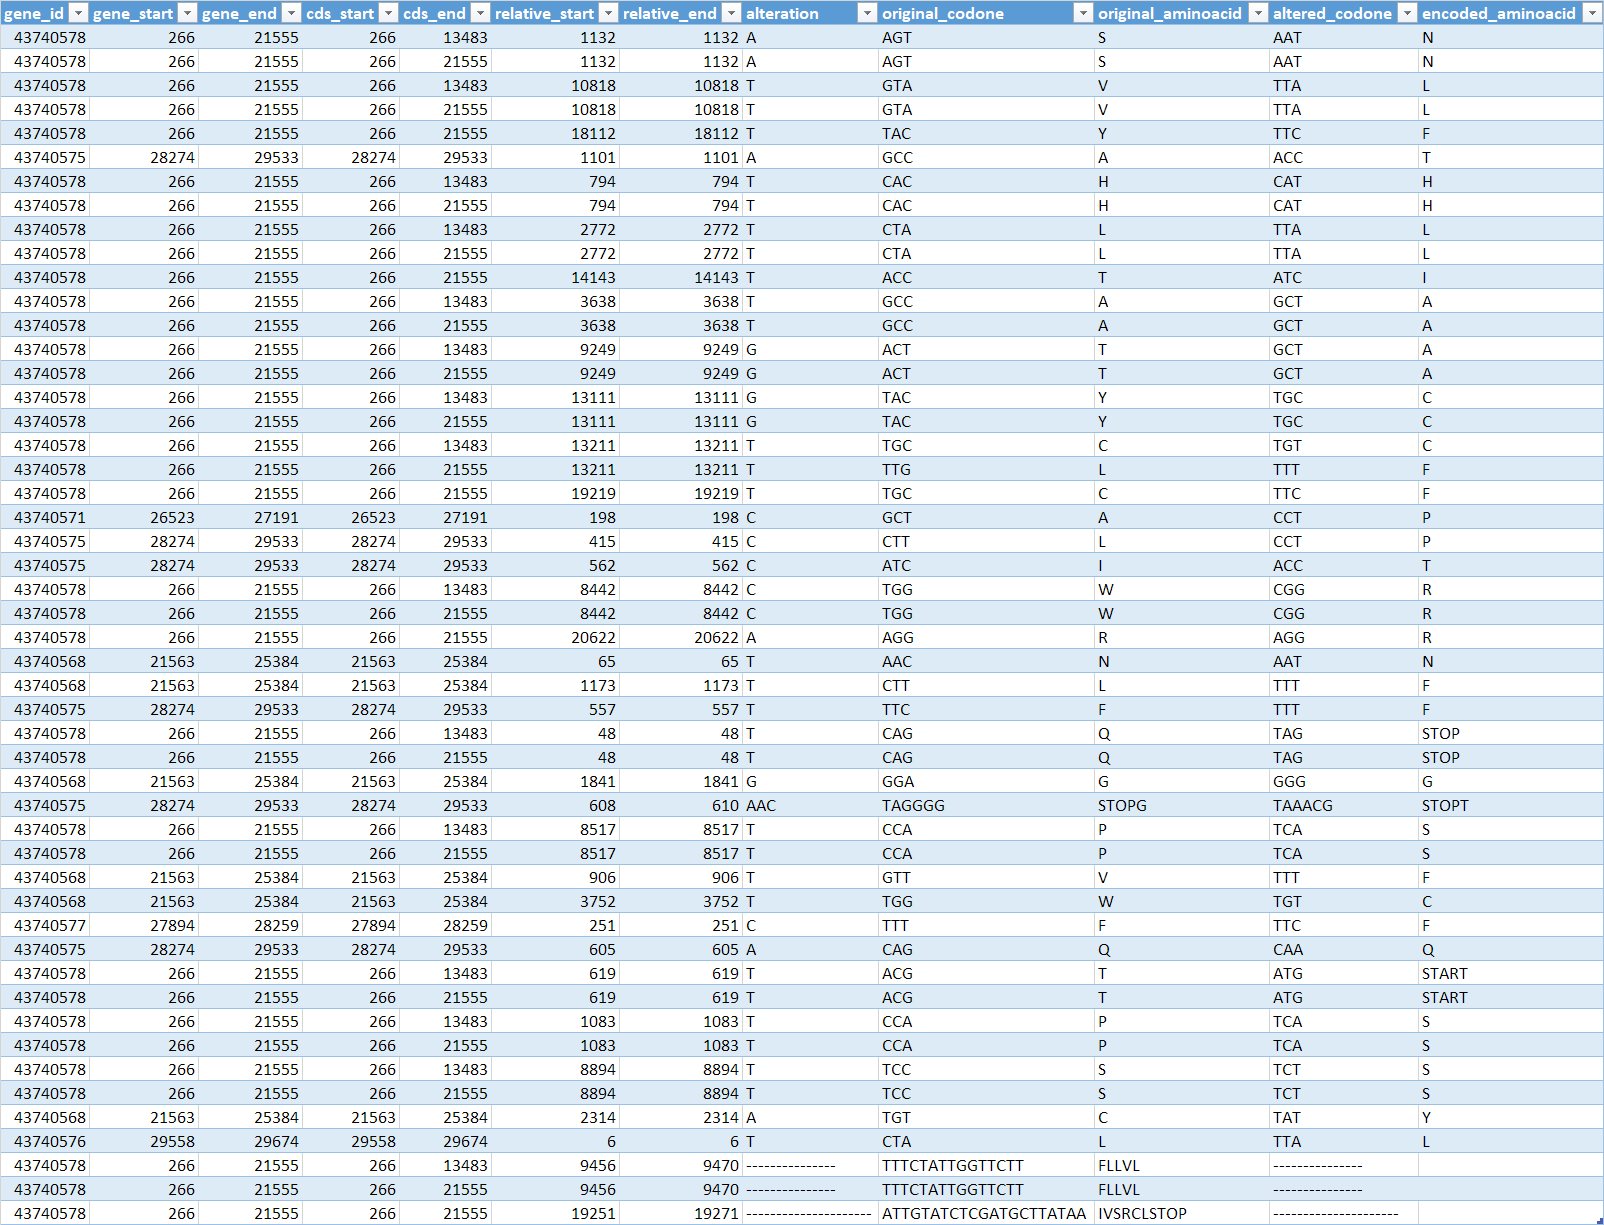
\includegraphics[width=1\linewidth]{alteration-table.png}}
  \caption{Tabella di output delle alterazioni}
  \label{fig:alteration_table}
\end{sidewaysfigure}

\newpage
\section{Output}
Come riportato in \cref{fig:alteration_table} la maggior parte delle alterazioni coinvolgono un singolo codone e quelli ottenuti rimangono traducibili.

In alcuni casi, l'amminoacido risultante dalla traduzione dell'alterazione non viene modificato.\hspace{1mm}La maggior parte delle variazioni si concentrano nel gene \lstinline{ORF1ab} identificato da \lstinline{gene_id = 43740578}.

Le ultime righe della tabella riportano delle alterazioni che determinano la cacellazione di alcune basi rispetto alla sequenza reference.
Queste sono relative solo alla sequenza \lstinline{MT262993.1} e si pensa possano derivare da un errore in fase di sequenziamento.


\section{Analisi dei risultati e conclusioni}
Le alterazioni appartenenti a geni si concentrano per quasi i tre quarti del totale sul gene \lstinline{ORF1ab}. Variazioni minori  seguito dai geni \lstinline{gene_name=S} e \lstinline{gene_name=N} (12\% ciascuno) e che gli altri siano quasi invariati.
Un'analisi finale si trova nella terza e ultima parte del progetto.

\begin{figure}[H]
  \makebox[\textwidth][c]{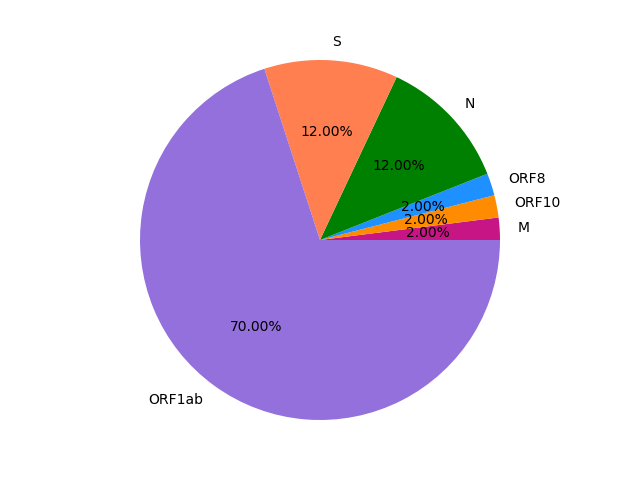
\includegraphics[width=1.1\linewidth]{plot-variations-per-gene.png}}
  \caption{Tipologia di variazioni}
  \label{fig:jalview-inner}
\end{figure}

\subsection{Divisone del lavoro}
Durante la realizzazione del progetto entrambi i componenti del gruppo hanno partecipato attivamente alla sua realizzazione. In particolare:
\begin{itemize}
  \item \textbf{Edoardo Silva} si è occupato principalmente di recuperare e gestire l'output JSON del progetto1 e delle funzioni di supporto.
  \item \textbf{Davide Marchetti} si è occupato principalmente di generare i file di output e correggere le porzioni di codice relative alle letture delle reference.
  \item Entrambi hanno lavorato alla creazione ed elaborazione dei dati, alla matrice delle mutazioni e le traduzioni di quest'ultime.
\end{itemize}


\end{document}